\documentclass[xcolor=svgnames,dvipsnames,table, hyperref=pdftex, mathserif, presentation]{beamer}
\usepackage{amsmath,amssymb,amsfonts,amsthm}
\usepackage{ctex}
\usepackage{graphics}
\usepackage{graphicx}
\usepackage{xcolor}
\usepackage{wasysym}
\usepackage{bbm}
\usepackage{url}
\usepackage{beamerleanprogress}
\usepackage{tikz-dependency}
\usepackage{tikz-qtree}

\usetheme{CambridgeUS}
%\usetheme{Pittsburgh}
\usecolortheme{orchid} % seahorse  orchid rose
\setbeamertemplate{blocks}[rounded][shadow=true]
\AtBeginSection[]{%
  \begin{frame}<beamer>
    \frametitle{Outline}
      \tableofcontents[current] 
    \end{frame}
  \addtocounter{framenumber}{-1}% If you don't want them to affect the slide number
}
\AtBeginSubsection[]
{
  \begin{frame}
  \frametitle{Outline}
    \tableofcontents[currentsection,currentsubsection]
  %\tableofcontents[sectionstyle=show/hide,subsectionstyle=hide/show/hide]
  \end{frame}
  \addtocounter{framenumber}{-1}% If you don't want them to affect the slide number
}
\newcommand{\setof}[1]{\ensuremath{\left \{ #1 \right \}}}
\newcommand{\tuple}[1]{\ensuremath{\left \langle #1 \right \rangle }}
\newcommand{\red}[1]{\textcolor{red}{#1}}
\newcommand{\brown}[1]{\textcolor{brown}{#1}}
\newcommand{\green}[1]{\textcolor{green}{#1}}
\newcommand{\blue}[1]{\textcolor{blue}{#1}}
\newcommand{\cyan}[1]{\textcolor{cyan}{#1}}

%gets rid of navigation symbols
\setbeamertemplate{navigation symbols}{}

\begin{document}

\title[Paraphrase]{Dynamic Pooling and Unfolding Recursive Autoencoders for Paraphrase Detection (NIPS2011)}

\institute[icst@pku]{
  
}
\author[Zhe Han]{\\ Zhe Han \\ 1401214342\\ iampkuhz@gmail.com
}

\frame[t,plain]{ \titlepage } % [t,plain]

\frame{
  \frametitle{ Outline  }
  
   \begin{itemize}
  \item Paraphrase identification(复述检测)
    \begin{itemize}
     \item Definition
     \item Common methods
    \end{itemize}

  \item 本文的方法
    \begin{itemize}
      \item Recursive Autoencoder
      \item Dynamic Pooling
    \end{itemize}

  \item 实验效果
    \begin{itemize}
    \item 实验效果
    \item 分析, 对比其他任务
    \end{itemize}
  \end{itemize}

}

\frame{
  \frametitle{Paraphrase identification}
  
  \begin{itemize}
   \item definition
      \begin{itemize}
       \item 给定一组句子, 判断其是否是复述
	  \begin{itemize}
	   \item binary classification
	  \end{itemize}

      \end{itemize}
      
    \item Microsoft Research Paraphrase Corpus (MSRP)
	\begin{itemize}
	 \item train: 4,076 sentence pairs (2,753 positive: 67.5 \%)
	 \item test: 1,725 sentence pairs (1,147 positive: 66.5 \%)
	 \item 2个标注者, 83\%的一致性, 第三个人更正
	\begin{block}{Sample data}
	 \begin{itemize}
	 	 \item Sentence 1: Amrozi accused his brother, whom he called "the witness", of deliberately distorting his evidence.
	       \item Sentence 2: Referring to him as only "the witness", Amrozi accused his brother of deliberately distorting his evidence.
	       \item Class: 1 (true paraphrase)
	 \end{itemize}
	\end{block}
	
	\end{itemize}
  \end{itemize}

}


\frame{
    \frametitle{Paraphrase identification}
    \begin{itemize}
     \item Common methods
	\begin{itemize}
	  \item lexical features
	      \begin{itemize}
	       \item n-gram features, skip-gram fatures, ...
	      \end{itemize}

	  \item semantic features
	      \begin{itemize}
	       \item POS tag, wordnet similarity, dependency tree relation, ...
	      \end{itemize}

	  \item classification
	      \begin{itemize}
	       \item SVM, voted classifications
	      \end{itemize}
	\end{itemize}
    
    \item Challenge
	\begin{itemize}
	 \item 没有提取句子的全局信息( dependency features利用不足)
	 \item 对句子涵义的特征提取不足(没有真正理解句子)
	\end{itemize}

    \end{itemize}

}

\frame{
\begin{footnotesize}
    \frametitle{This paper}
    \begin{block}{Main method}
	\begin{itemize}
	 \item 利用NYT新闻训练每个单词的向量(100维)
	 \item 对于每个句子(多个单词向量)采用训练一个递归的自动编码机, 得到一个句子级别的语义向量. 
	 \item 通过判断两个句子的语义向量的相似性得到语义相似性特征
	\end{itemize}
    \end{block}

    \begin{itemize}
	 \item 递归的自动编码机(Unfolding Recursive Autoencoder) 
	    \begin{itemize}
	     \item 抽取句子的语义向量, 得到语法数上每个节点(单词, 短语)的向量
	    \end{itemize}
	 \item Dynamic Pooling
	    \begin{itemize}
	     \item 对于长度变化的两个句子, 抽取固定维数的特征
	    \end{itemize}

	\end{itemize}
\end{footnotesize}
}

\frame{
\begin{footnotesize}
    \frametitle{Unfolding Recursive Autoencoder}
    \begin{itemize}
     \item Autoencoder
	\begin{itemize}
	 \item 不对所有层的参数进行一次性的优化, 而是一层层的优化
	 \item 对于每一层的输入, 跑一层神经网络, 得到输入的特征表示(认知过程)
	 \item 对于之前得到的特征再跑一层神经网络, 我们希望输入和输出尽可能相似(生成过程)
	\end{itemize}

     \item Recursive Autoencoder
	\begin{itemize}
	 \item \footnotesize{进一步的, 对于深层的网络(语法树), 递归使用同一个简单的Autoencoder}
	\end{itemize}
	
	
	\begin{figure}[H]
	 \begin{minipage}[h]{0.33\linewidth}
\centering
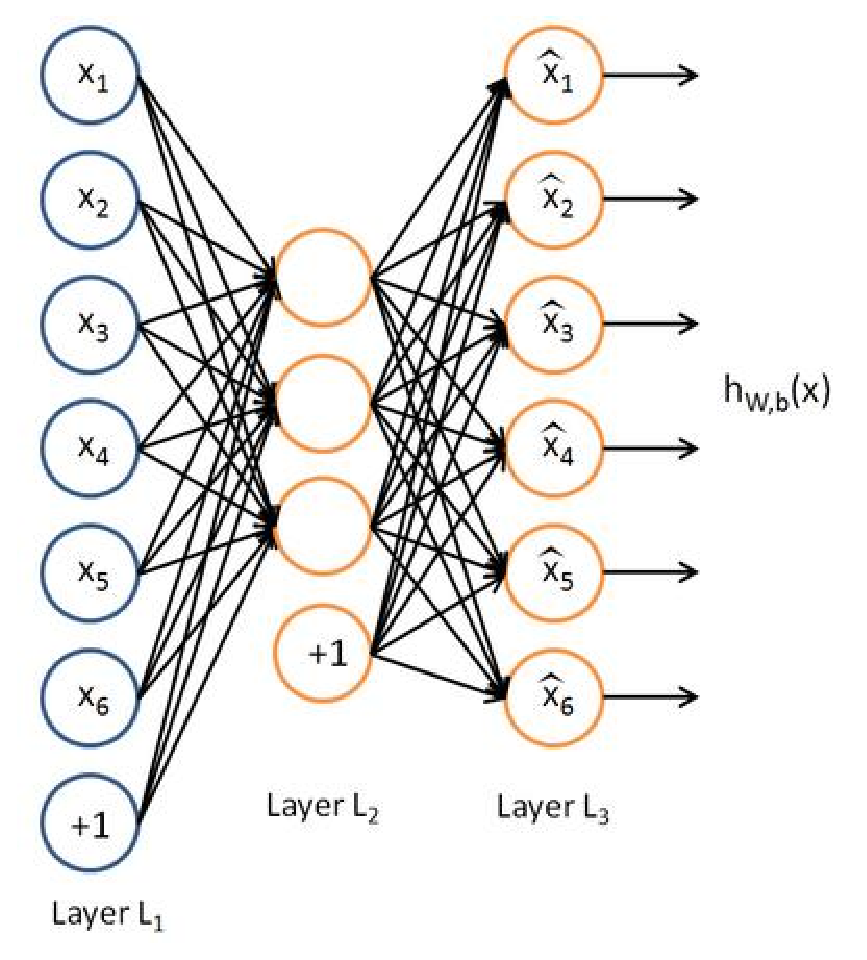
\includegraphics[width=0.8\textwidth]{Autoencoder.eps}
\caption{\begin{tiny}
          constituency tree
         \end{tiny}}
\end{minipage}
\begin{minipage}[h]{0.5\linewidth}
\centering
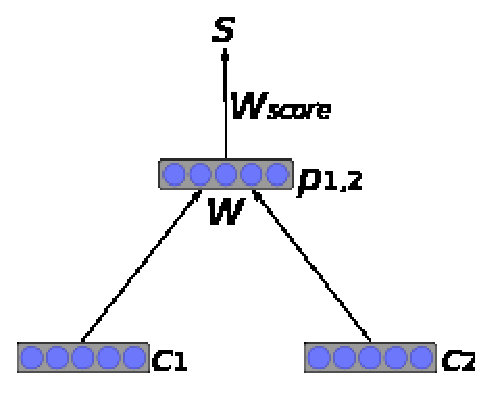
\includegraphics[width=0.5\linewidth]{rAutoencoder.eps}
\begin{tiny}
 \caption{\begin{tiny}
          dependency tree
         \end{tiny}}
\end{tiny}

\end{minipage}
	\end{figure}
	
    \end{itemize}
\end{footnotesize}
}

\frame{
     \frametitle{Unfolding Recursive Autoencoder}
  \begin{figure}[h]
  \centering
  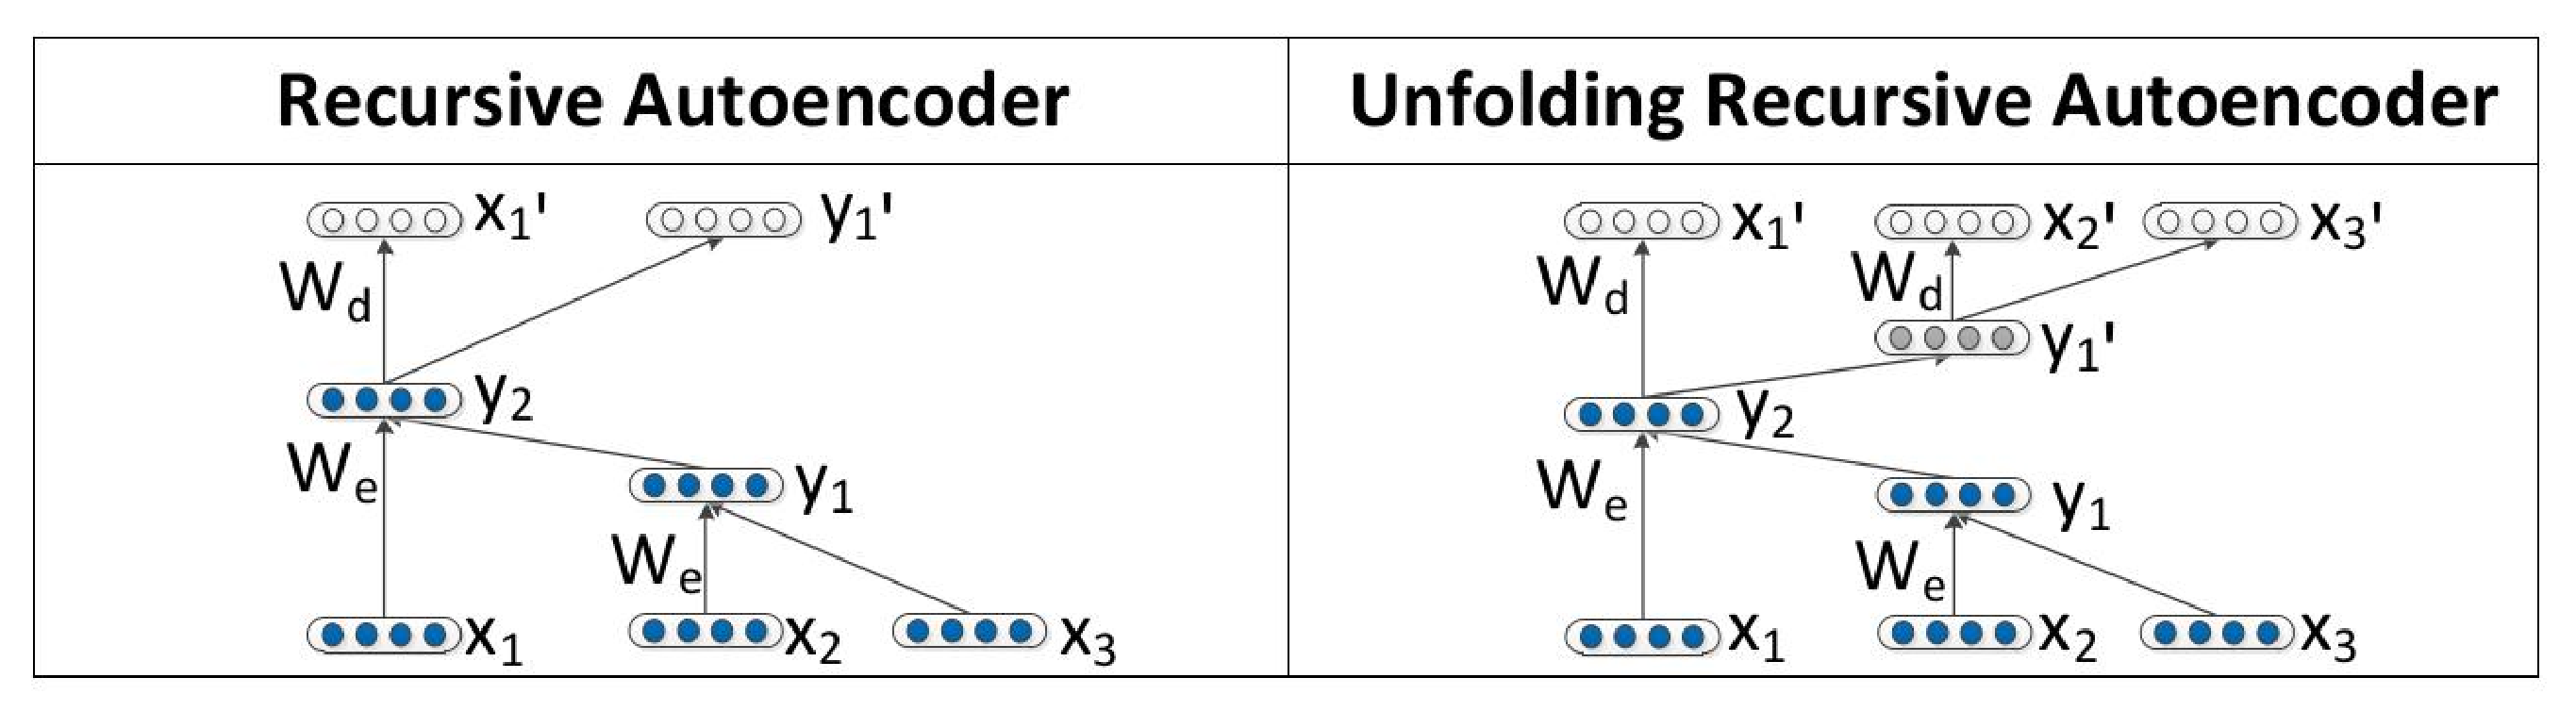
\includegraphics[width=0.8\textwidth]{uRAE}
  \end{figure}
  
  \begin{itemize}
      \item Recursive Autoencoder
      \item Comparison (on $y_2 -> x_1y_1$)
	  \begin{itemize}
	   \item Neural network
	      \begin{itemize}
	       \item minimum $\parallel y_2'-y_2\parallel$
	      \end{itemize}
	
	   \item Recursive Autoencoder
	   \begin{itemize}
	    \item minimum $\parallel[x_1';y_1']-[x_1;y_1]\parallel $
	   \end{itemize}
 
	   \item Unfolding Recursive Autoencoder
	      \begin{itemize}
	       \item  minimum $\parallel[x_1';x_2';...;x_j']-[x_1;x_2;...;x_j]\parallel $
	      \end{itemize}
	  \end{itemize}
      
    \end{itemize}
}

\frame{
    \frametitle{Unfolding Recursive Autoencoder(RAE)}
  \begin{figure}[h]
  \centering
  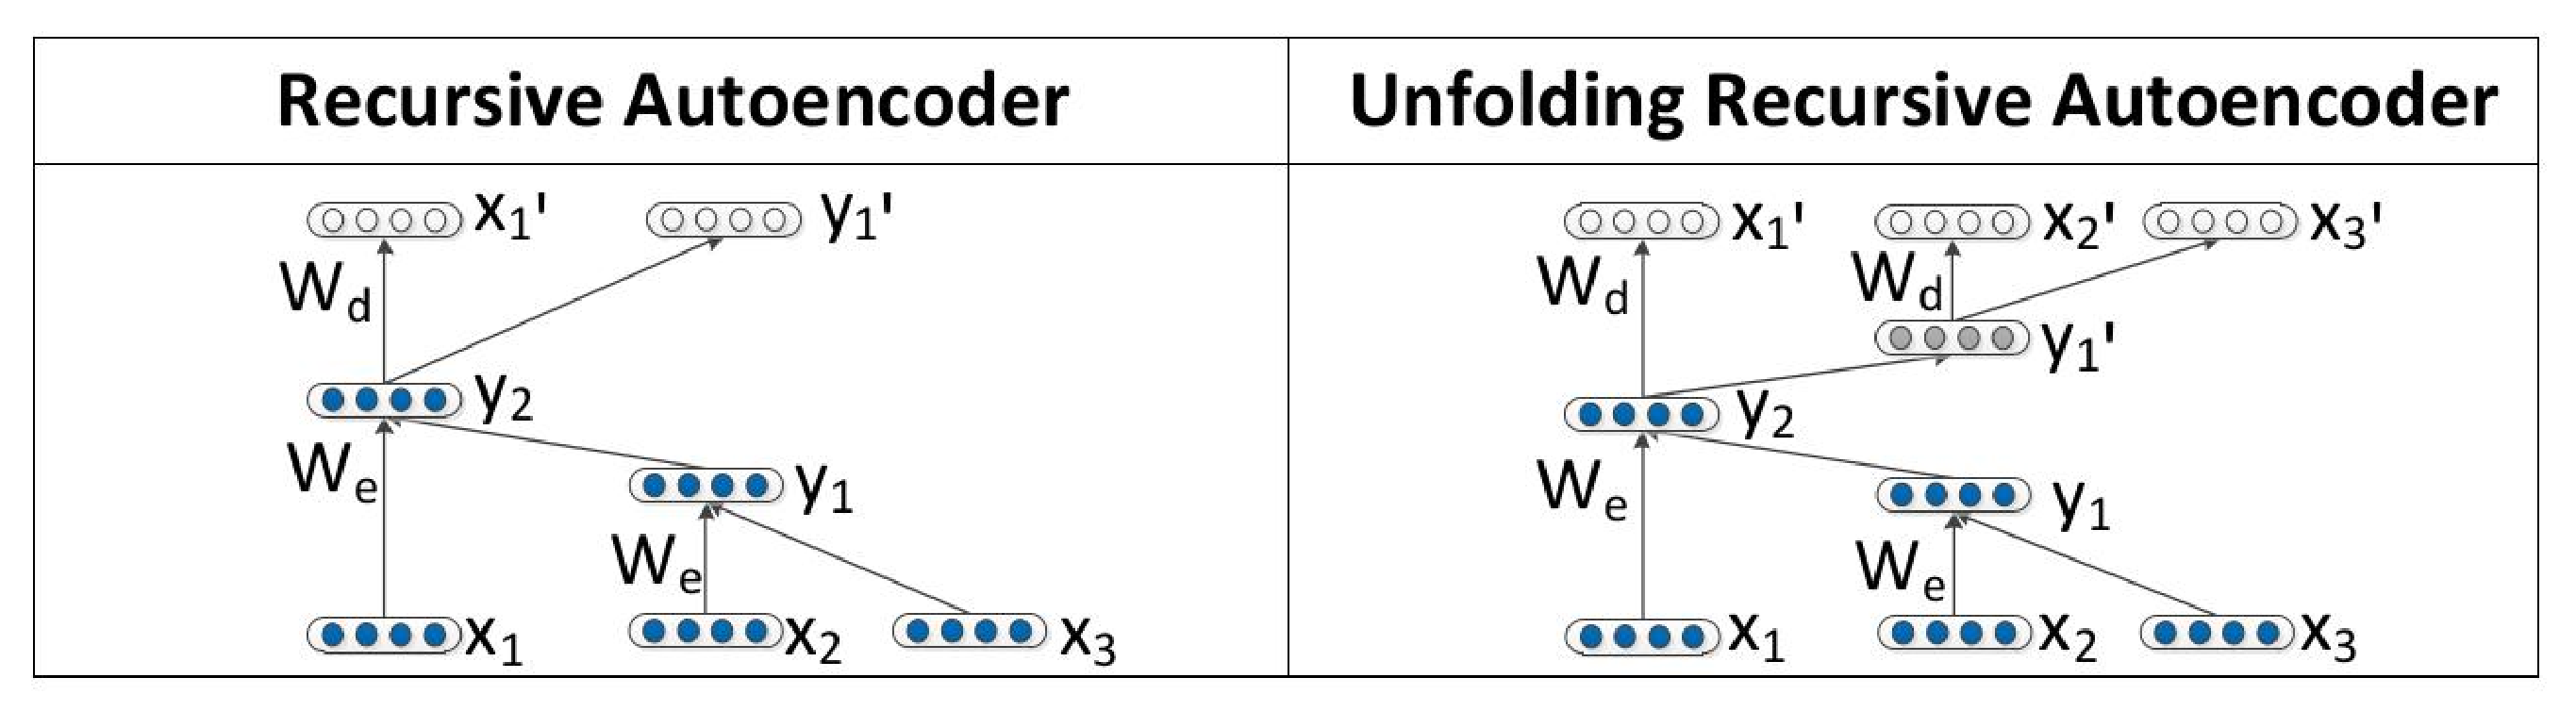
\includegraphics[width=0.6\textwidth]{uRAE}
  \end{figure}
  \begin{tiny}
%uRAE 和 RAE类似, 我们通过解释RAE过程来说明生成句子的语义向量的过程   
  \end{tiny}

    \begin{itemize}
     \item 初始化每个单词的向量
	\begin{itemize}
	 \item 100维,可以通过word2vec或glove实现
	\end{itemize}
     \item 得到句子的constituency tree
	\begin{itemize}
	 \item 二叉
	\end{itemize}

	\begin{figure}
	 \begin{minipage}[h]{0.43\linewidth}
\centering
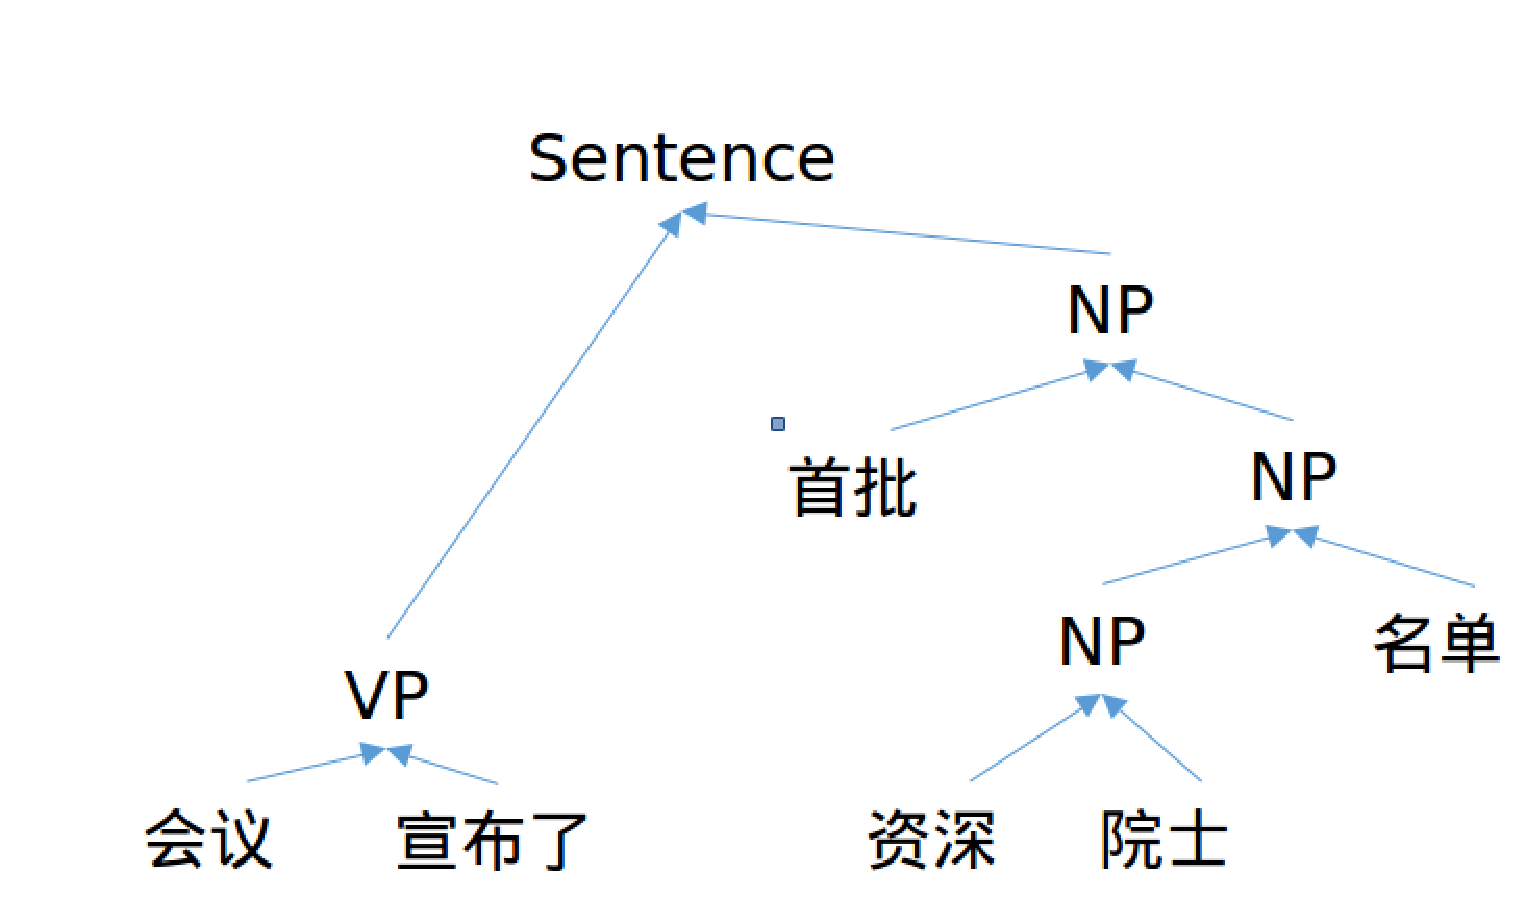
\includegraphics[width=0.8\textwidth]{cTree.eps}
\caption{\begin{tiny}
          constituency tree
         \end{tiny}}
\end{minipage}
\begin{minipage}[h]{0.45\linewidth}
\centering
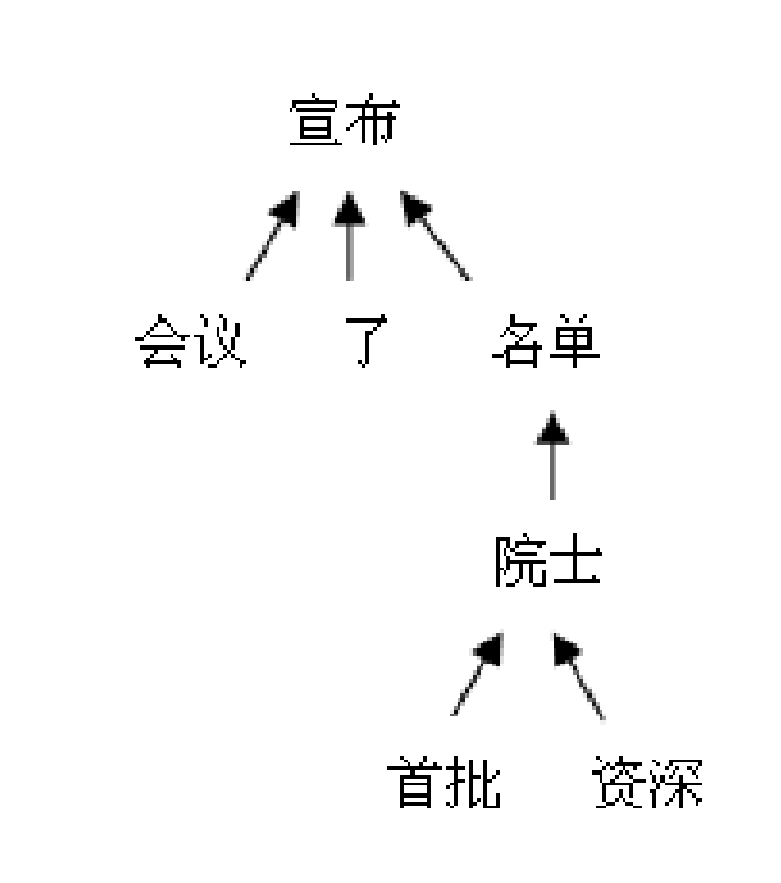
\includegraphics[width=0.45\linewidth]{dTree.eps}
\begin{tiny}
 \caption{\begin{tiny}
          dependency tree
         \end{tiny}}
\end{tiny}


\end{minipage}
	\end{figure}
    \end{itemize}

}

\frame{
   \frametitle{Unfolding Recursive Autoencoder(uRAE)}
  \begin{figure}[h]
  \centering
  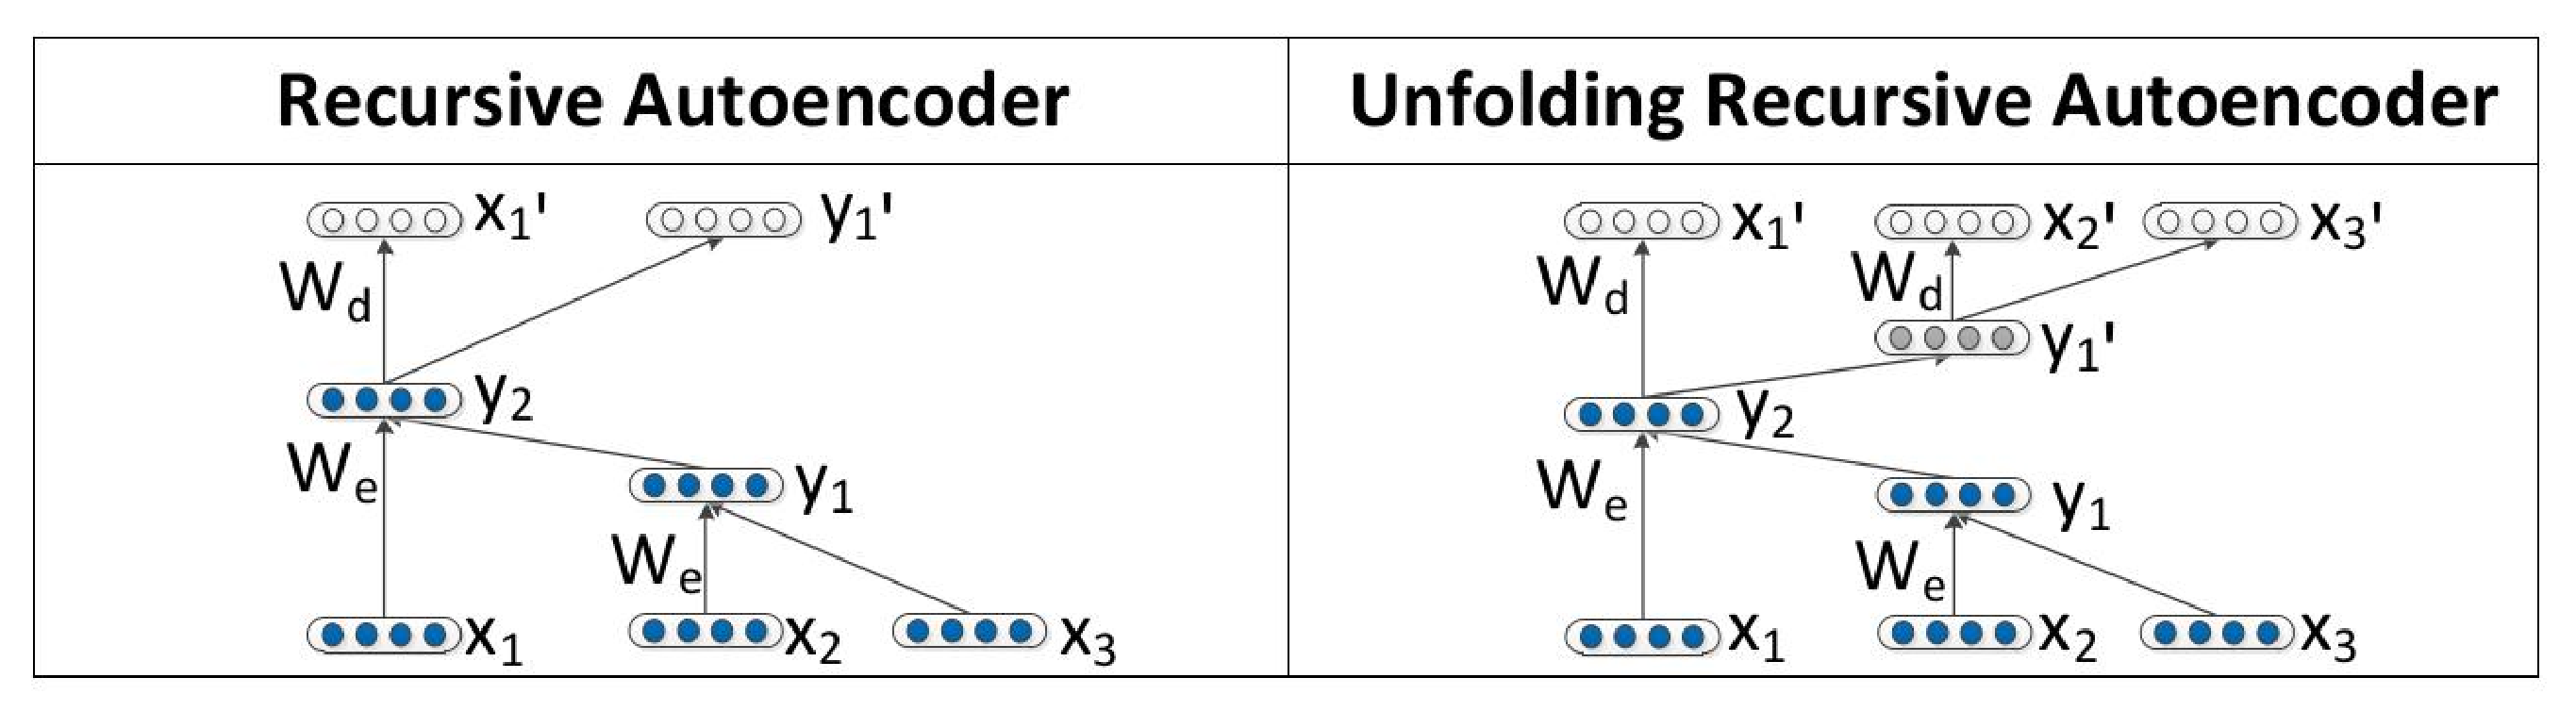
\includegraphics[width=0.6\textwidth]{uRAE}
  \end{figure}
  
   \begin{itemize}
    \item 损失函数
	\begin{itemize}
	 \item 对于左图的关系:$y_1\to x_2x_3,y_2\to x_1y_1$
	  \begin{itemize}
	   \item 先正向(自底向上):对于规则$p\to c_1c_2$,有$p=f(W_e[c_1,c_2]+b)$,带入两个关系$y_1,y_2$依次实例
	   \item 后逆向(自顶向下):对于上面的规则$[c_1';c_2']=f(W_dp+b_d)$,如果$c_1';c_2'$不是叶节点,递归做
	  \end{itemize}
	\item 损失函数为$E_rec(y_{(i,j)})=\parallel[x_i;..;x_j]-[x_i';...;x_j']\parallel^2$
	  \begin{itemize}
	   \item 对比RAE:逆向时只做一层,损失函数为 $E_rec(p)=\parallel[c_1;c_2]-[c_1';c_2']\parallel^2$
	  \end{itemize}

	\item 梯度下降求解$W_e,b,W_d,b_d$
	\end{itemize}

   \end{itemize}
}

\frame{
  \frametitle{Dynamic Pooling}
  \begin{figure}[h]
  \centering
  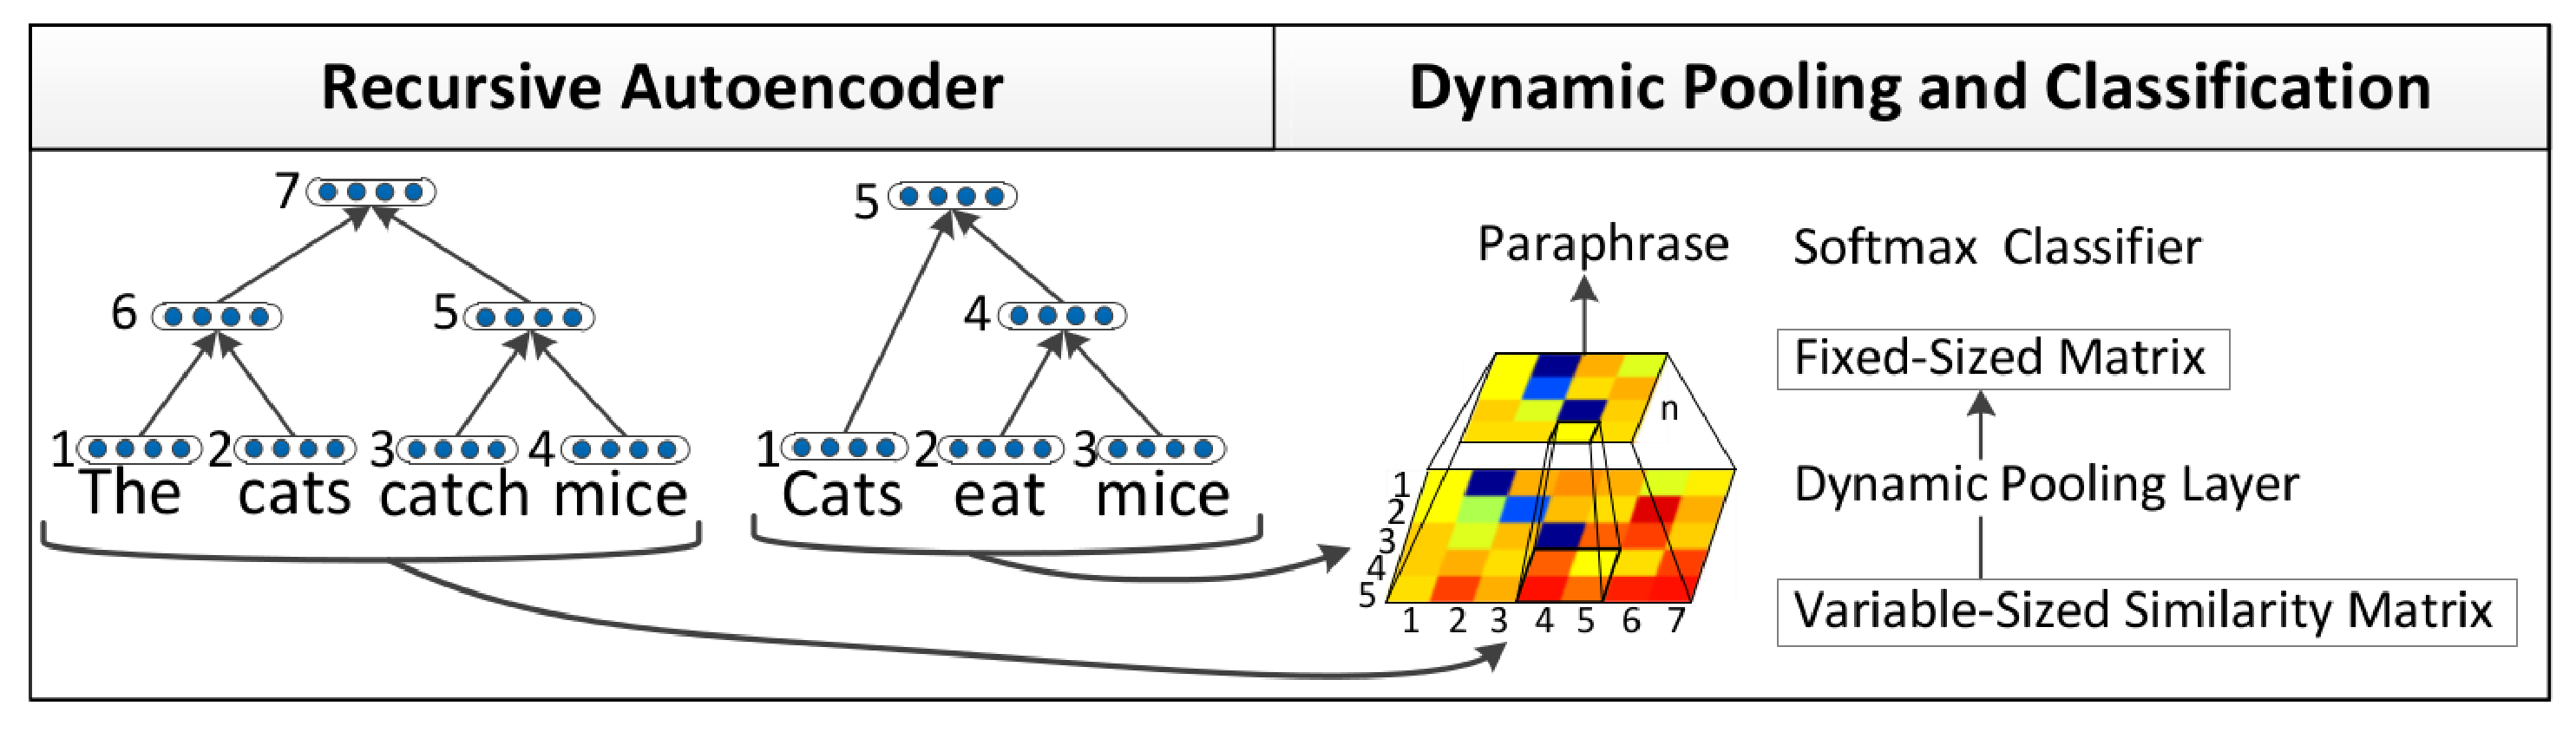
\includegraphics[width=0.8\textwidth]{DynamicPooling}
  \end{figure}
  
  
  \begin{itemize}
   \item motivation
      \begin{itemize}
       \item 如何对两个长度变化的句子(而且很可能不一样)抽取固定维数的特征?
       \begin{itemize}
        \item 长度为n的句子,cTree有(2n-2)个节点,不同的句子对应的维数不同
       \end{itemize}

       \item polling! 把不同长度的句子压缩(扩张)到相同的维数
	  \begin{itemize}
	   \item (实验验证,15维最好,略低于平均句子长度)
	  \end{itemize}
       
      \end{itemize}
  \end{itemize}

}

\frame{
  \frametitle{Dynamic Pooling}
  \begin{figure}[h]
  \centering
  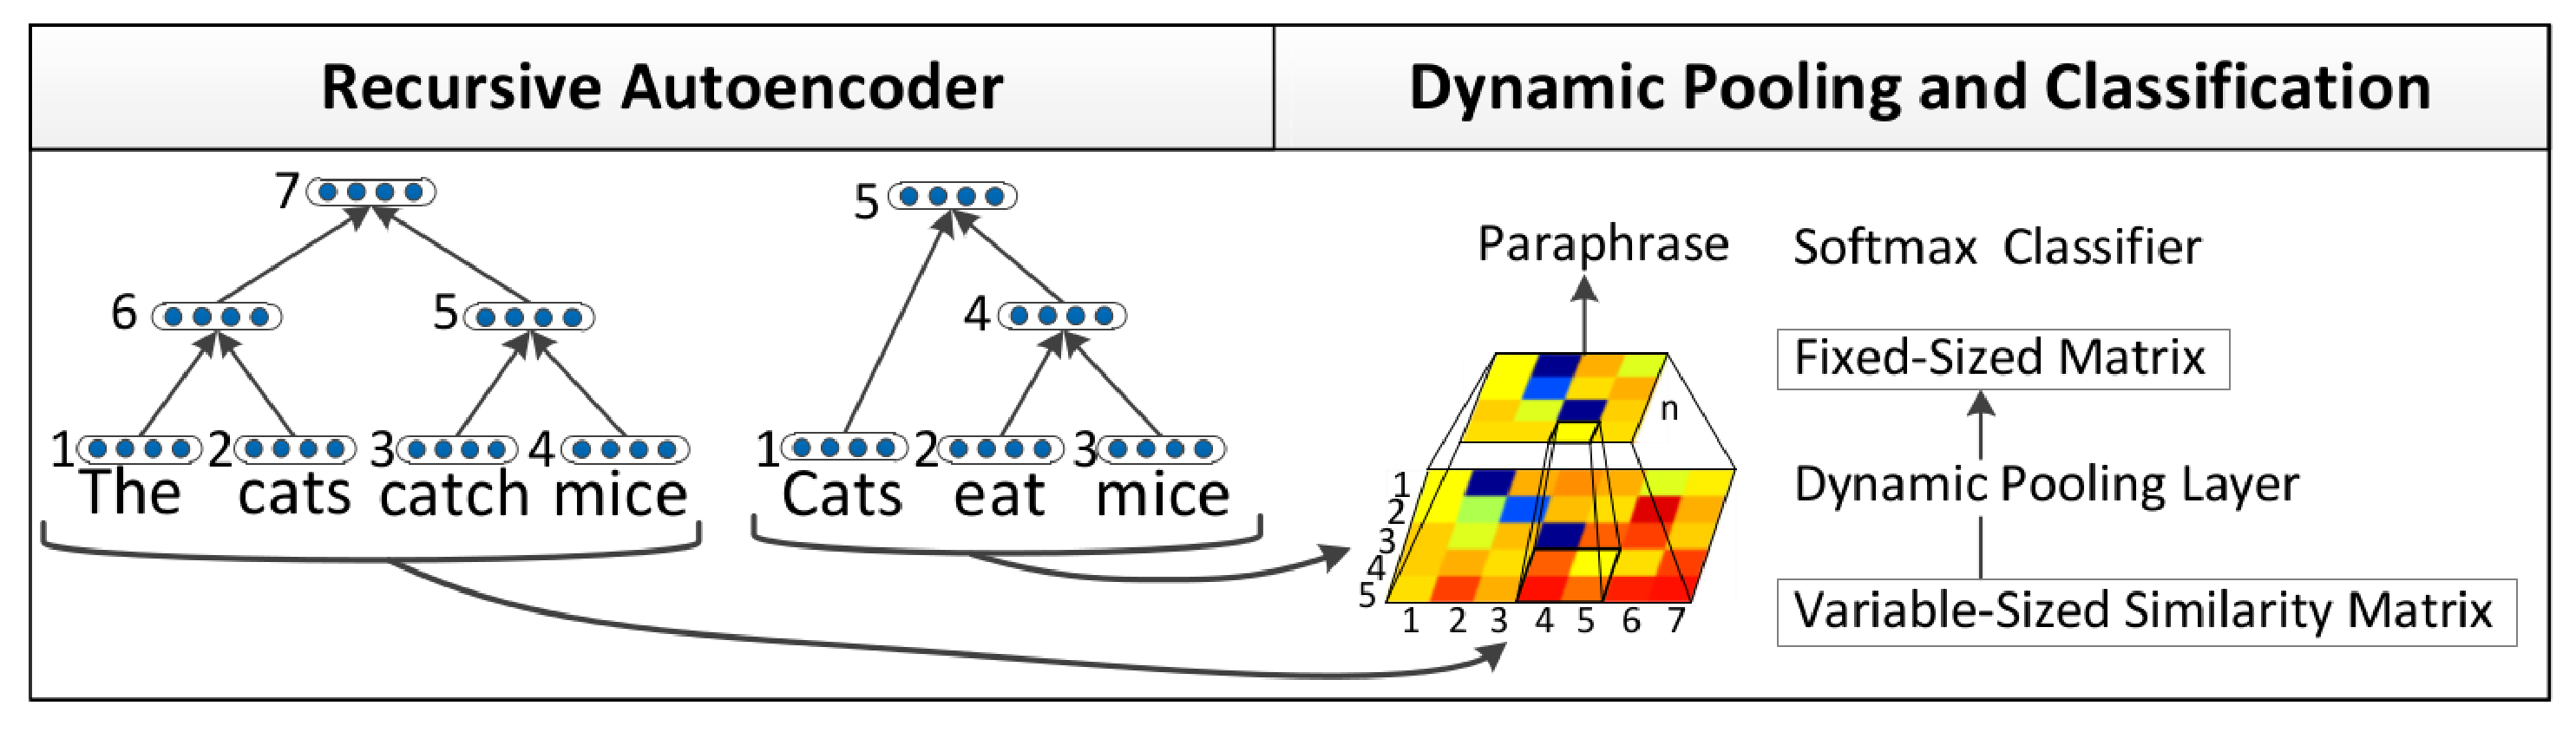
\includegraphics[width=0.8\textwidth]{DynamicPooling}
  \end{figure}
  
  \begin{itemize}
   \item method
	\begin{itemize}
	 \item 将向量“等”分成k(=15)份,原来的(2n-1)*(2m-1)维向量分成$k^2$块,从每块中提取最小值作为该块的值
	    \begin{itemize}
	     \item 平均值掩盖了特异的特征,最小值(or最大值?)更容易体现其中一个的特异特征
	    \end{itemize}

	\end{itemize}

  \end{itemize}
  
  \begin{figure}[h]
  \centering
  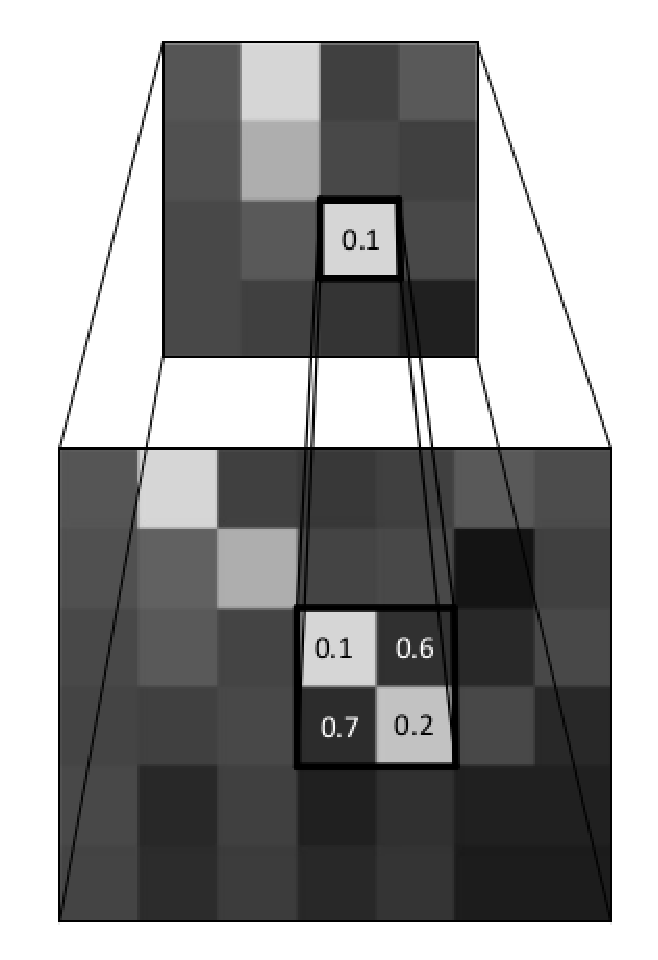
\includegraphics[height=0.4\textheight, angle=90]{pollingMin}
  \end{figure}

}

\frame{
  \frametitle{Experiment result(2011)}
  \begin{itemize}
   \item features
      \begin{itemize}
       \item Dynamic pollinged matrix S$(\mathbb{R}^{15*15})$, three number features, sentence length, string mathes
      \end{itemize}
  \end{itemize}

  \begin{figure}
   \centering
  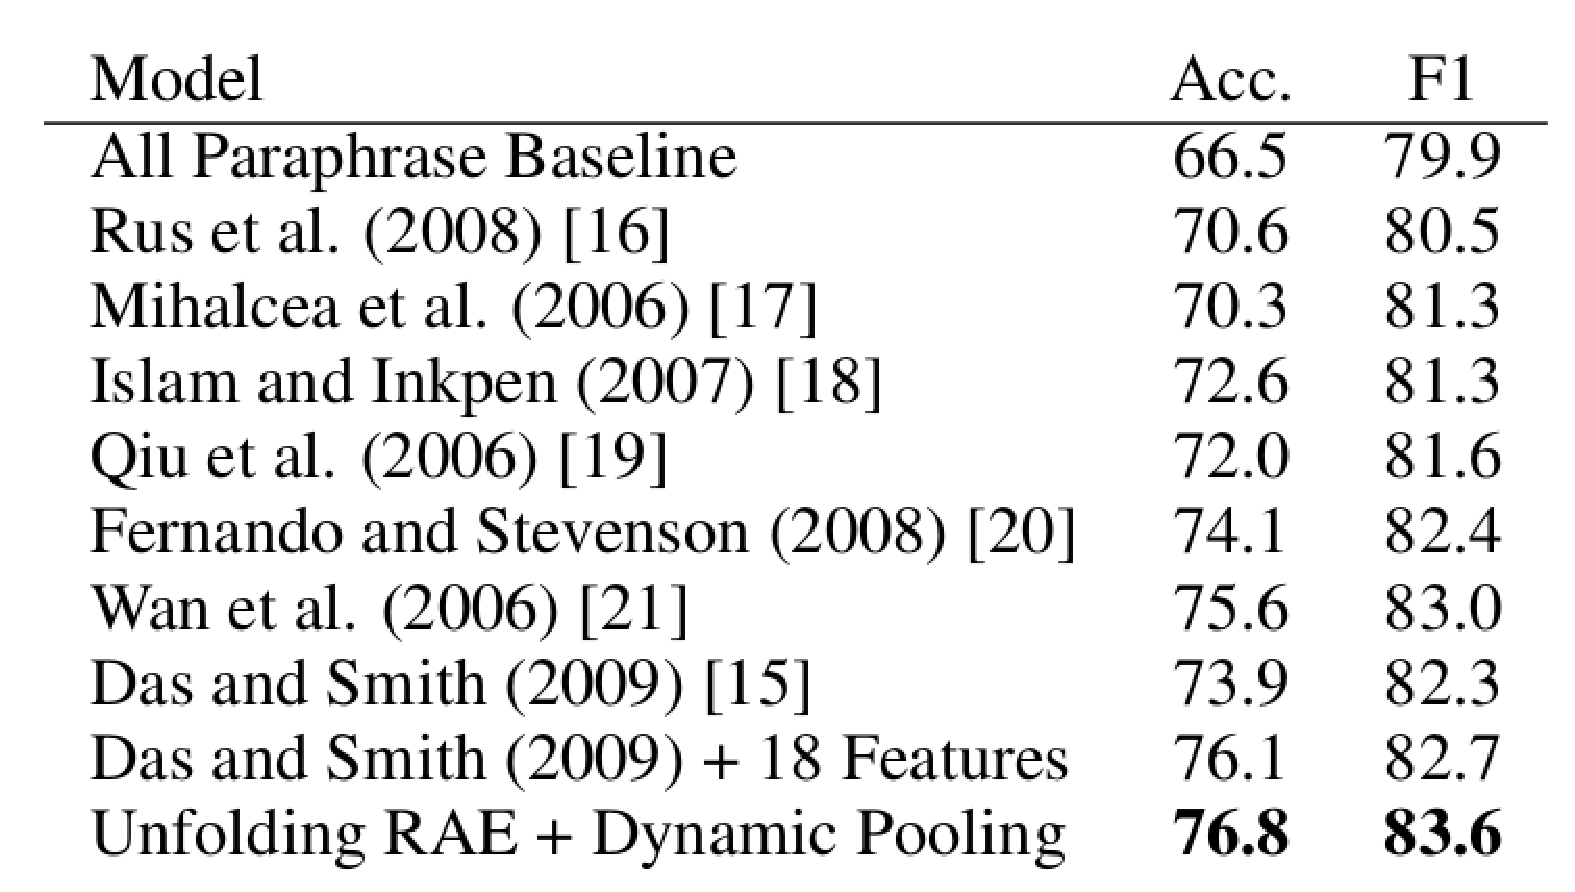
\includegraphics[height=0.3\textwidth]{ResultAccu}

  \end{figure}
  
  \begin{figure}
  \centering
  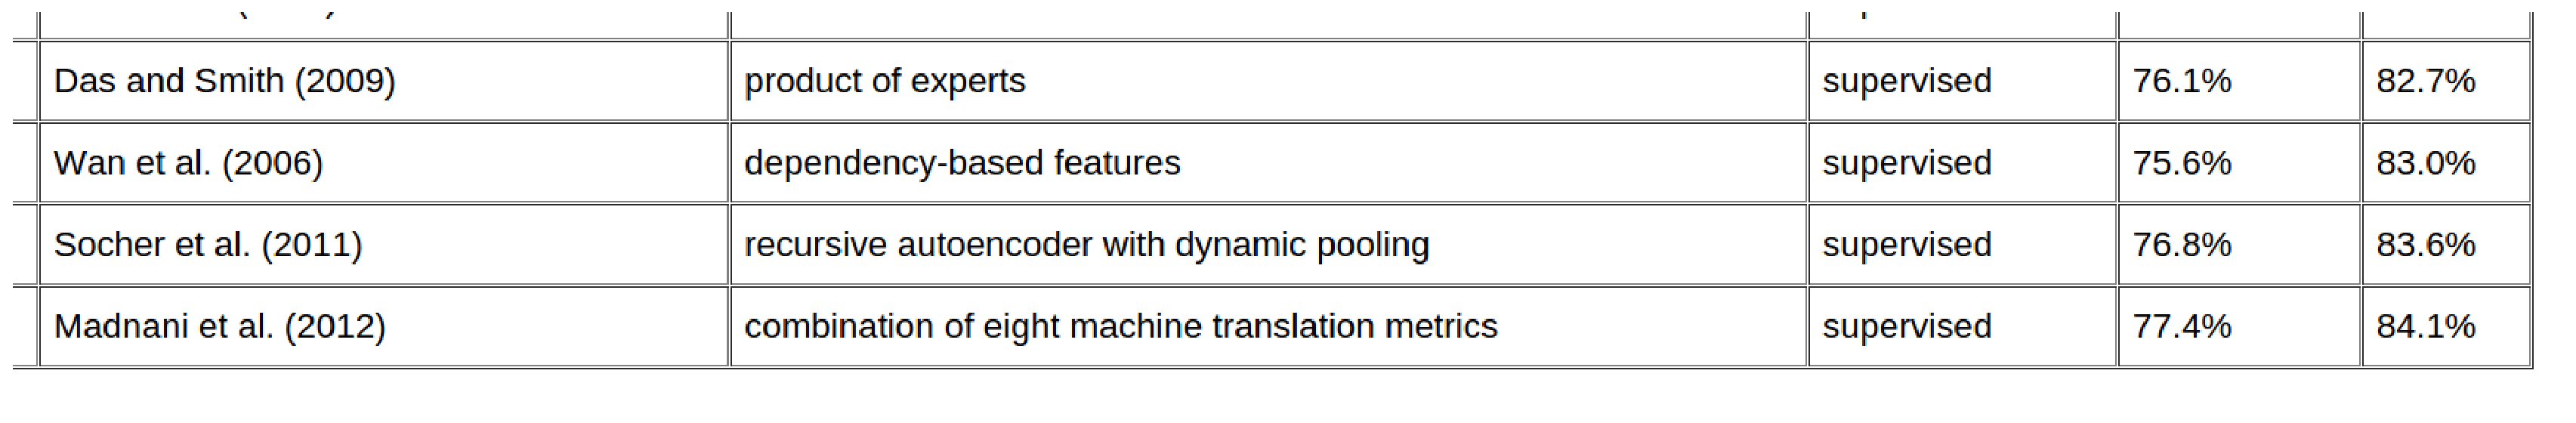
\includegraphics[width=0.8\textwidth]{StateOfArt}
  \end{figure}
  
}

\frame{
  \frametitle{Analysis}
  \begin{itemize}
   \item QA
   \begin{itemize}
   \item Why use uRAE instead of RAE or Recursive.avg?
      \begin{itemize}
       \item 多个单词组成的句子(高层节点),需要更多的单词信息,RAE只关心最近的2个儿子节点
       \item Recursive.avg:两个儿子向量的平均忽视了结构关系
       \item 实验证明,Recursive.avg找不出来;RAE对2个单词组成的短语,识别其近义词效果很好;uRAE对于2-3个单词组成的短语的效果很好,甚至5个单词组成的短语有些也可以正确找到。
      \end{itemize}
      
  \begin{figure}
  \centering
  \includegraphics[width=0.65\textwidth]{Comp}
  \end{figure}
  \end{itemize}

  \end{itemize}

}

\frame{
  \frametitle{Analysis \& Summary}
  \begin{itemize}
   \item QA
      \begin{itemize}
       \item Does deep RAE improve the acc?
	\begin{itemize}
	 \item No. Slow and worse. 过拟合,和两个儿子非常像,忽视了更深的叶节点,长的短语(>2)效果非常差
	\end{itemize}
      \end{itemize}
    
    \item Summary
	\begin{itemize}
	\item 非常漂亮
	    \begin{itemize}
	    \item 特征的类别很少(4类), 语义信息起到了很大的作用
	    \item (我自己)21种feature,77.2\% (单一SVM:76.8\%)
	    \item 之前的文章,鲜有使用semantic info。而且一般只用了wordNet的同义词/上位词,结合dependency pair进行判断,局限于单个label,没有全局信息,对整体的效果提升没有这么显著
	    \end{itemize}
	\item 利用文章的句子语义表述方法
	    \begin{itemize}
	    \item 维基百科谓词归一:根据描述句子的相似性判断谓词是否表达同一意思
	    \end{itemize}

	\end{itemize}

  \end{itemize}

}
\end{document}
